%
% Main document
% ===========================================================================
% This is part of the document "Project documentation template".
% Authors: brd3, kaa1
%
%---------------------------------------------------------------------------
\documentclass[
    a4paper,                % paper format
    10pt,                   % fontsize
    %twoside,               % double-sided
    openright,              % begin new chapter on right side
    notitlepage,            % use no standard title page
    parskip=half,           % set paragraph skip to half of a line
]{scrreprt}                 % KOMA-script report
%---------------------------------------------------------------------------
\raggedbottom{}
%\KOMAoptions{cleardoublepage=plain}         % Add header and footer on blank pages


% Load Standard Packages:
%---------------------------------------------------------------------------
\usepackage{scrpage2}
\usepackage[standard-baselineskips]{cmbright}
\usepackage[ngerman]{babel}                                             % german hyphenation
\usepackage[utf8]{inputenc}                                             % UTF-8 input encoding
\usepackage[T1]{fontenc}                                                % hyphenation of words with ä,ö and ü
\usepackage{textcomp}                                                   % additional symbols
\usepackage{etoolbox}                                                   % color manipulation of header and footer
\usepackage{graphicx}                                                   % integration of images
\usepackage{float}                                                      % floating objects
\usepackage[font={footnotesize,it}]{caption}                                                    % for captions of figures and tables
\usepackage{booktabs}                                                   % package for nicer tables
\usepackage{tocvsec2}                                                   % provides means of controlling the sectional numbering
\usepackage[square,sort,comma,authoryear]{natbib}                           % provides various citation styles
\usepackage{wrapfig}                                                    % provides floating of text around images
\usepackage{nameref}                                                    % provides printing names of references
\usepackage{colortbl}                                                   % Colored tables
\usepackage{scrhack}                                                    % Remove float errors and warnings
\usepackage{pgfgantt}                                                   % Provides GANTT charts
\usepackage{array}
%---------------------------------------------------------------------------

% Load Math Packages
%---------------------------------------------------------------------------
\usepackage{amsmath}                                                    % various features to facilitate writing math formulas
\usepackage{amsthm}                                                     % enhanced version of latex's newtheorem
\usepackage{amsfonts}                                                   % set of miscellaneous TeX fonts that augment the standard CM
\usepackage{amssymb}                                                    % mathematical special characters
\usepackage{exscale}                                                    % mathematical size corresponds to textsize
%---------------------------------------------------------------------------

% Package to facilitate placement of boxes at absolute positions
%---------------------------------------------------------------------------
\usepackage[absolute]{textpos}
\setlength{\TPHorizModule}{1mm}
\setlength{\TPVertModule}{1mm}
%---------------------------------------------------------------------------   
% PDF als Anhang                 
\usepackage{pdfpages}
% Definition of Colors
%---------------------------------------------------------------------------
\RequirePackage{color}                          % Color (not xcolor!)
\definecolor{linkblue}{rgb}{0,0,0.8}            % Standard
\definecolor{darkblue}{rgb}{0,0.08,0.45}        % Dark blue
\definecolor{bfhgrey}{rgb}{0.41,0.49,0.57}      % BFH grey
%\definecolor{linkcolor}{rgb}{0,0,0.8}              % Blue for the web- and cd-version!
\definecolor{linkcolor}{rgb}{0,0,0}                 % Black for the print-version!

%---------------------------------------------------------------------------

% Load listings package
% which provides source code formatting
%---------------------------------------------------------------------------
\usepackage{listings}                                                   % provides source code formatting
% Define XML colors
\lstdefinelanguage{XML}
{
  basicstyle=\ttfamily\footnotesize,
  morestring=[b]'',
  moredelim=[s][\bfseries\color{maroon}]{<}{\ },
  moredelim=[s][\bfseries\color{maroon}]{</}{>},
  moredelim=[l][\bfseries\color{maroon}]{/>},
  moredelim=[l][\bfseries\color{maroon}]{>},
  morecomment=[s]{<?}{?>},
  morecomment=[s]{<!--}{-->},
  commentstyle=\color{codecommentcolor},
  stringstyle=\color{darkblue},
  identifierstyle=\color{red}
}
% Change captions of listings
\renewcommand{\lstlistingname}{Auflistung}
\renewcommand{\lstlistlistingname}{Auflistungsverzeichnis}
%---------------------------------------------------------------------------

% Hyperref Package (Create links in a pdf)
%---------------------------------------------------------------------------
\usepackage[
    pdftex,ngerman,bookmarks,plainpages=false,pdfpagelabels,
    backref = {false},                                      % No index backreference
    colorlinks = {true},                  % Color links in a PDF
    hypertexnames = {true},               % no failures "same page(i)"
    bookmarksopen = {true},               % opens the bar on the left side
    bookmarksopenlevel = {0},             % depth of opened bookmarks
    pdftitle = {Template für Bachelor Thesis},      % PDF-property
    pdfauthor = {brd3},                           % PDF-property
    pdfsubject = {LaTeX Template},        % PDF-property
    linkcolor = {linkcolor},              % Color of Links
    citecolor = {linkcolor},              % Color of Cite-Links
    urlcolor = {linkcolor},               % Color of URLs
]{hyperref}
%---------------------------------------------------------------------------
% Set up page dimension
%---------------------------------------------------------------------------
\usepackage{geometry}
\geometry{a4paper,
    left=28mm,
    right=15mm,
    top=30mm,
    headheight=20mm,
    headsep=10mm,
    textheight=242mm,
    footskip=15mm
}
%---------------------------------------------------------------------------

% Makeindex Package
%---------------------------------------------------------------------------
\usepackage{makeidx}                                % To produce index
\makeindex                                      % Index-Initialisation
%---------------------------------------------------------------------------

% Glossary Package
%---------------------------------------------------------------------------
% the glossaries package uses makeindex
% if you use TeXnicCenter do the following steps:
%  - Goto "Ausgabeprofile definieren" (ctrl + F7)
%  - Select the profile "LaTeX => PDF"
%  - Add in register "Nachbearbeitung" a new "Postprozessoren" point named Glossar
%  - Select makeindex.exe in the field "Anwendung" ( ..\MiKTeX x.x\miktex\bin\makeindex.exe )
%  - Add this [ -s "%tm.ist" -t "%tm.glg" -o "%tm.gls" "%tm.glo" ] in the field "Argumente"
%
% for futher informations go to http://ewus.de/tipp-1029.html
%---------------------------------------------------------------------------
\usepackage[nonumberlist]{glossaries}
%\usepackage[xindy,nonumberlist]{glossaries}
\newglossaryentry{OWL}{name={OWL},description={
    Web Ontology Language;
    Ontologiesprache für das semantische Web.
    Mit dieser Sprache können Ontologien beschrieben werden.
}}

\makeglossaries{}
%---------------------------------------------------------------------------

% Intro:
%---------------------------------------------------------------------------
%\begin{document}                                % Start Document
\settocdepth{section}                                                       % Set depth of toc
\pagenumbering{roman}                                                       
%---------------------------------------------------------------------------

\providecommand{\titel}{Volume ray casting --- basics \& principles}
                  % Titel der Arbeit aus Datei titel.tex lesen
\providecommand{\versionnumber}{0.1}		%  Hier die aktuelle Versionsnummer eingeben
\providecommand{\versiondate}{{\today}}		%  Hier das Datum der aktuellen Version eingeben
                % Versionsnummer und -datum aus Datei version.tex lesen

% Set up header and footer
%---------------------------------------------------------------------------

\deftripstyle{newlayout}
  [0pt] % no header line
  [0pt] % no footer line
  {}
  {}
  {}
  {\color{bfhgrey} \footnotesize \titel, Version \versionnumber, \versiondate}
  {}
  {\color{bfhgrey} \thepage}

\pagestyle{newlayout}
% use "pagestyle" also on chapter starting pages 
\renewcommand{\chapterpagestyle}{newlayout}
\renewcommand{\chaptermark}[1]{\markboth{\thechapter.  #1}{}}
\renewcommand*{\headfont}{\normalfont}
\renewcommand*{\footfont}{\normalfont}
%---------------------------------------------------------------------------

% We need this as mr. gantt chart (teh package..) thinks text should be gray..
\color{black}

\begin{document}

% Title Page and Abstract
%---------------------------------------------------------------------------
% -*- coding: UTF-8 -*-
% vim: autoindent expandtab tabstop=4 sw=4 sts=4 filetype=tex
% chktex-file 27 - disable warning about missing include files
% chktex-file 36 - disable put space in front of parentheses warning

\begin{titlepage}

    % BFH-Logo absolute placed at (28,12) on A4 and picture (16:9 or 15cm x 8.5cm)
    % Actually not a realy satisfactory solution but working.
    %---------------------------------------------------------------------------
    \setlength{\unitlength}{1mm}
    \begin{textblock}{20}[0,0](28,12)
        
\includegraphics[scale=1.0]{img/BFH_Logo_B.png}
    \end{textblock}

    \begin{textblock}{154}(28,48)
        \begin{picture}(150,2)
            \put(0,0){\color{bfhgrey}\rule{150mm}{2mm}}
        \end{picture}
    \end{textblock}

    \begin{textblock}{154}[0,-0.2](26,40)
        \centering
        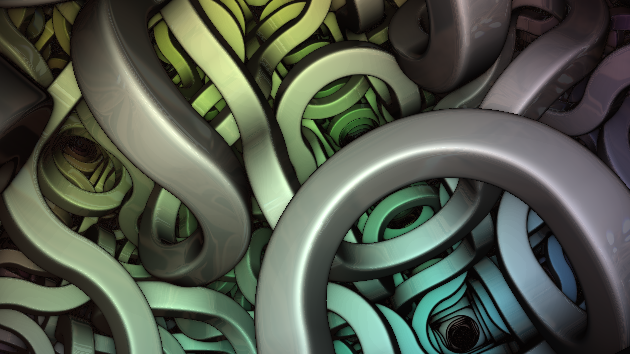
\includegraphics[scale=0.6]{img/logo.png}
    \end{textblock}

    \begin{textblock}{154} (28,135)
        \begin{picture}(150,2)
            \put(0,0){\color{bfhgrey}\rule{150mm}{2mm}}
        \end{picture}
    \end{textblock}
    \color{black}

    \begin{flushleft}
        \vspace*{120mm}
        \fontsize{26pt}{28pt}\selectfont
        \titel{}\\
        \vspace{3mm}
        \fontsize{14pt}{16pt}\selectfont
        \textbf{Projektarbeit 1} \\
        \vspace{6mm}

        \textbf{MTE7101} \\
        \vspace{3mm}

        \begin{textblock}{150} (28,215)
            \fontsize{10pt}{17pt}\selectfont
            \begin{tabbing}
            xxxxxxxxxxxxxxx   \= xxxxxxxxxxxxxxxxxxxxxxxxxxxxxxxxxxxxxxxxxxxxxxx \kill
            Studiengang:      \> Informatik                                         \\
            Autor:            \> Sven Osterwalder\protect\footnotemark[1]{}         \\
            Betreuer:         \> Prof.~Claude Fuhrer\protect\footnotemark[2]{} \\
            Datum:            \> \vhCurrentDate{}\\
            Version:          \> \vhCurrentVersion\\
            \end{tabbing}
        \end{textblock}
    \end{flushleft}
    \footnotetext[1]{sven.osterwalder@students.bfh.ch}
    \footnotetext[2]{claude.fuhrer@bfh.ch}

    \begin{textblock}{150} (28,280)
        \noindent
        \color{bfhgrey}\fontsize{9pt}{10pt}\selectfont
        Berner Fachhochschule | Haute école spécialisée bernoise | Bern University of Applied Sciences
        \color{black}\selectfont
    \end{textblock}

    \vfill
    
\includegraphics[height=\baselineskip]{img/by-sa}\\ \small{\sffamily{Licensed under the Creative Commons Attribution-ShareAlike 3.0 License}}

\end{titlepage}
          % activate for Titelseite mit Bild
\cleardoublepage{}
\phantomsection{}
% -*- coding: UTF-8 -*-
% vim: autoindent expandtab tabstop=4 sw=4 sts=4 filetype=tex
% chktex-file 27 - disable warning about missing include files

% Versionenkontrolle :
% -----------------------------------------------

\chapter*{}
\label{chap:versionen}

\begin{versionhistory}
    \vhEntry{0.1}{25.09.2015}{SO}{Initiale Erstellung des Dokumentes}
    \vhEntry{0.2}{27.09.2015}{SO}{Entwickeln einer initialen Struktur,
        Dokumentaufbau, Entwicklung Kapitel~\ref{chap:procedure}, Beschreibung von
        Ray Tracing in Kapitel~\ref{chap:theoretical_background}, Hinzufügen des
        Kapitels~\ref{chap:20_administrative}, Einführen von TODO-Notizen
    }
    \vhEntry{0.3}{29.09.2015}{SO}{Einführen von Meeting
        Minutes~\ref{chap:10_meeting_minutes}, Erweitern des
        Kapitels~\ref{chap:theoretical_background} um Belechtungsmodelle, Beschreiben von
        lokalen Beleuchtungsmodellen
    }
    \vhEntry{0.4}{04.10.2015}{SO}{Hinzufügen von Standards und
        Richtlinien~\ref{subsec:standards_guidelines}, Erweitern des
        Kapitels~\ref{chap:theoretical_background} um globale
        Belechtungsmodelle~\ref{subsec:global_illumination_models} sowie Ray
        Casting~\ref{subsec:ray_casting}, Entfernen der Schriftart `cmbright', Hinzufügen
        des Kapitels über (implizite) Oberflächen~\ref{sec:surfaces}
    }
    \vhEntry{0.5}{11.10.2015}{SO}{Neuordnung des
        Kapitels~\ref{chap:theoretical_background}: Hinzufügen des Kapitels über Ray
        Tracing~\ref{sec:ray_casting_tracing} sowie über Darstellung von impliziten
        Oberflächen~\ref{sec:description_implicit_surfaces}
    }
    \vhEntry{0.6}{14.10.2015}{SO}{Hinzufügen von TODO-Notizen, Anpassung der
        Textdarstellung in Formeln
    }
    \vhEntry{0.7}{16.10.2015}{SO}{Hinzufügen einer Illustration des
        Phong-Beleuchtungmodelles in Kapitel~\ref{subsec:local_illumination_models},
        Abarbeiten von TODO-Notizen in diversen Kapiteln, Erweitern des Kapitels über
        (implizite) Oberflächen~\ref{sec:surfaces}
    }
    \vhEntry{0.8}{17.10.2015}{SO}{Hinzufügen einer Illustration des Ray Tracing
        Algorithmus in Kapitel~\ref{subsec:global_illumination_models}
    }
    \vhEntry{0.9}{19.10.2015}{SO}{Beginn Kapitel über Rendering von impliziten
        Oberflächen~\ref{sec:rendering_implicit_surfaces}
    }
    \vhEntry{0.10}{21.10.2015}{SO}{Erweiterung Kapitel über Rendering von
        impliziten Oberflächen, Einführung Kapitel über die Umsetzung eines
        Prototypen~\ref{chap:prototype}
    }
    \vhEntry{0.11}{24.10.2015}{SO}{Umstrukturierung des Dokumentes, Anpassung
        der Dokumentvorlage, Nachführen der Versionshistorie, Ausführen der
        Meeting Minutes vom 18.10.2015, Erstellen der Vorlage für Meeting
        Minutes vom 25.10.2015
    }
    \vhEntry{0.12}{31.10.2015}{SO}{Nachführen der Versionshistorie, Ausführen der
        Meeting Minutes vom 25.10.2015, Erstellen der Vorlage für Meeting
        Minutes vom 02.11.2015, Erweiterung des
        Kapitels~\ref{chap:prototype}, Abarbeiten von TODO-Notizen
    }
    \vhEntry{0.13}{07.11.2015}{SO}{Ausführen der Meeting Minutes vom
        02.11.2015, Erweiterung des Kapitels~\ref{chap:prototype}
    }
    \vhEntry{0.14}{15.11.2015}{SO}{Erarbeiten des
        Kapitels~\ref{sec:rendering_implicit_surfaces_shadows},
        Erweiterung des Kapitels~\ref{chap:prototype} um weiche Schatten, 
        Erstellen und Hinzufügen von Bildmaterial zu Kapiteln~\ref{subsec:ray_marching}
        und~\ref{subsec:sphere_tracing}.
    }
    \vhEntry{0.15}{29.11.2015}{SO}{Komplette Überarbeitung des Bildmaterials zu
        Kapiteln~\ref{subsec:ray_marching} und~\ref{subsec:sphere_tracing}.
    }
    \vhEntry{0.16}{06.12.2015}{SO}{Nachführen von Meeting Minutes und der
        Versionierung. Überarbeiten des Zeitplanes, weiter Überarbeitung des
        Bildmaterials. Hinzufügen des Kapitels~\ref{sec:shading}, Hinzufügen
        einer Einleitung zu Kapitel~\ref{chap:theoretical_background}.
    }
\end{versionhistory}

\phantomsection{}
\cleardoubleemptypage{}
\setcounter{page}{1}
\cleardoublepage{}
\phantomsection{}
\cleardoubleemptypage{}
%---------------------------------------------------------------------------

% Make sure Umlauts are getting displayed correctly.
\lstset{literate=%
    {Ö}{\textcolor{black}{\"O}}1
    {Ä}{{\"A}}1
    {Ü}{{\"U}}1
    {ß}{{\ss}}1
    {ü}{{\"u}}1
    {ä}{{\textcolor{black}{\"a}}}1
    {ö}{{\textcolor{black}{\"o}}}1
    {~}{{\textasciitilde}}1
    {?}{{\textcolor{black}{?}}}1
}

% Table of contents
%---------------------------------------------------------------------------
\tableofcontents
\cleardoublepage{}
%---------------------------------------------------------------------------

% Main part:
%---------------------------------------------------------------------------
\pagenumbering{arabic}
% -*- coding: UTF-8 -*-
% vim: autoindent expandtab tabstop=4 sw=4 sts=4 filetype=tex
% chktex-file 27 - disable warning about missing include files

\chapter{Einleitung}
\label{chap:10_introduction}

Seit dem Bestehen moderner Computer existiert auch die Computergrafik. Ziel der Computergrafik ist es unter Anderem den dreidimensionalen Raum auf eine zweidimensionale Fläche abzubilden, da die Ausgabe meist auf den zweidimensionalen Raum limitiert ist.

Dabei wird zwischen statischen Bildern und dynamischen Bildern unterschieden. Statische Bilder werden bei Bedarf dargestellt und ändern sich in der Regel nicht. Dynamische Bilder können sich hingegen ständig ändern und müssen --- bedingt durch das menschliche Auge --- mit 25 Bildern pro Sekunde ausgegeben werden. Es bestand bereits früh das Bestreben möglichst eine realistische Darstellung zu erhalten. Eine Darstellung also, die möglichst nahe an der menschlichen Wahrnehmung liegt.

Im Laufe der Zeit entstanden verschiedene Ansätze um eine solche Darstellung zu bieten. Ein Teilgebiet davon sind Beleuchtungsmodelle, welche die Beleuchtung einer Darstellung bzw.\ einer Szene berechnen. Dabei wird zwischen lokalen und globalen Beleuchtungsmodellen unterschieden.

Ein globales Beleuchtungsmodell ist Ray Tracing (zu deutsch Strahlenverfolgung), welches 1980 von Turner Whitted vorgestellt wurde wurde. Das Verfahren besticht durch seine Einfachheit und bietet dabei eine hohe Bildqualität mit perfekten Spiegelungen und Transparenzen. Mit entsprechenden Optimierungen ist das Verfahren auch relativ schnell.

Mit schnell ist dabei die Zeit gemeint, die benötigt wird um ein einzelnes Bild darzustellen. Möchte man jedoch eine Darstellung in Echtzeit erreichen, so war das Verfahren lange zu langsam.

Im Rahmen der Weiterentwicklung der Computer und vor allem durch die Weiterentwicklung der Grafikkarten (GPUs) ist Ray Tracing jedoch wieder in den Fokus der Darstellung von Szenen in Echtzeit gerückt.

Diese Projektarbeit stellt ein spezielles, auf Ray Tracing basierendes Verfahren zur Darstellung eines Bildes in Echtzeit vor: Das so Volume Ray Casting oder Sphere Tracing genannte Verfahren.

%---------------------------------------------------------------------------

% Glossary
%---------------------------------------------------------------------------
\cleardoublepage{}
\phantomsection{}
\addcontentsline{toc}{chapter}{Glossar}
\renewcommand{\glossaryname}{Glossar}
\glsaddall{}
\printglossaries{}
%---------------------------------------------------------------------------

% Bibliography
%---------------------------------------------------------------------------
%\cleardoublepage
\phantomsection{}
\addcontentsline{toc}{chapter}{Literaturverzeichnis}
\bibliographystyle{unsrtnat}
\bibliography{inc/bibliography}{}
\nocite{*} % TODO: Remove this when cites are in here
%---------------------------------------------------------------------------

% Listings
%---------------------------------------------------------------------------
%\cleardoublepage
\phantomsection{}
\addcontentsline{toc}{chapter}{Abbildungsverzeichnis}
\listoffigures
%\cleardoublepage
\phantomsection{}
\addcontentsline{toc}{chapter}{Tabellenverzeichnis}
\listoftables
%\cleardoublepage
\phantomsection{}
\addcontentsline{toc}{chapter}{Auflistungsverzeichnis}
\lstlistoflistings{}
%---------------------------------------------------------------------------

% Index
%---------------------------------------------------------------------------
%\cleardoublepage
%\phantomsection{}
%\addcontentsline{toc}{chapter}{Stichwortverzeichnis}
%\renewcommand{\indexname}{Stichwortverzeichnis}
%\printindex
%---------------------------------------------------------------------------

% Attachment:
%---------------------------------------------------------------------------
%\appendix
\settocdepth{section}
% -*- coding: UTF-8 -*-
% vim: autoindent expandtab tabstop=4 sw=4 sts=4 filetype=tex
% chktex-file 27

% In den Anhang fügen Sie ein:
%  * Details des Projektpans, falls vorhanden
%  * Resultate und Zwischenresultate in Funktion der Projektiterationen
%  * Pflichtenheft / Anforderungsspezifikation (Stand Ende dritter Woche)
%  * Angaben zum Projektrepository
%  * Sitzungsprotokolle, falls vorhanden
%  * Weiterführende Erläuterungen zu den verwendeten Technologien, falls nötig
%  * Benutzerhandbuch, falls vorhanden und sinnvoll, es hier aufzulisten
%  * Installations- und Betriebsdokument, falls vorhanden und sinnvoll, es hier aufzulisten
% Unterlassen Sie das Anfügen von Listings.

\appendix 
\begin{titlepage}
    \clearpage
    \vspace*{\fill}
    \begin{center}
        \begin{minipage}{.6\textwidth}
            \fontsize{26pt}{28pt}\selectfont
            \chapter*{Anhang}\label{chap:attachment}
            \addcontentsline{toc}{chapter}{Anhang}
        \end{minipage}
    \end{center}
    \vfill % equivalent to \vspace{\fill}
    \clearpage
\end{titlepage}

\newpage
 % -*- coding: UTF-8 -*-
% vim: autoindent expandtab tabstop=4 sw=4 sts=4 filetype=tex

\chapter{Meeting minutes}
\label{chap:10_meeting_minutes}

\VerbatimInput[label=20150921]{inc/static/attachment/minutes/20150921}



% \includepdfset{pagecommand={\thispagestyle{headings}}}
% \includepdf[pages=-, addtotoc={1,chapter,0,Anforderungsdokument,chap:anf},scale=0.95]{anhang/anforderungen.pdf}
% \newpage
% \includepdf[pages=-, addtotoc={1,chapter,0,Tutorial Wissensmodellierung,chap:tutorial},scale=0.95]{anhang/Tutorial.pdf}
% \newpage
% \input{anhang/schnipsel}
% \newpage
% \input{anhang/modellierung}
% \newpage
% \input{anhang/installationshandbuch}
% \newpage
% \includepdf[pages=-, addtotoc={1,chapter,0,Arbeitsjournal ,chap:arbeitsjournal},scale=0.95]{anhang/Journal.pdf}
% \newpage


%---------------------------------------------------------------------------

%---------------------------------------------------------------------------
\end{document}
